\chapter{AI Component Design}
\label{chap:ai-component-design} % Corrected label to be specific

\section{Business Context and AI Integration}
\label{section:business_context} % Kept original unique label
\usevar{\srsTitle} tackles the complex challenge of tracking individuals across multiple camera views in environments like campuses and factories. The core task requires recognizing and associating individuals as they move between potentially non-overlapping camera fields, often amidst changing appearances, viewpoints, lighting conditions, and occlusions. This inherent complexity and real-world variability make manual tracking labor-intensive, error-prone, and difficult to address effectively with traditional rule-based programming. Artificial Intelligence is therefore central to \usevar{\srsTitle}, providing the automation necessary to significantly improve this process.
The primary AI-driven workflow resides within the system's backend processing core, orchestrated by a service-oriented architecture. This workflow involves several key AI steps:
\begin{enumerate}
    \item \textbf{Person Detection:} Identifying individuals within each camera frame using high-performance detection models.
    \item \textbf{Intra-Camera Tracking:} Maintaining consistent temporary IDs for detected individuals within a single camera's view over consecutive frames, utilizing robust tracking algorithms.
    \item \textbf{Feature Extraction for Re-ID:} Generating unique appearance embeddings (features) from detected person images when necessary using discriminative feature extraction models.
    \item \textbf{Cross-Camera Re-Identification (Re-ID):} Matching these appearance embeddings across different camera views and time gaps to assign a persistent global identity, linking temporary tracks together.
    \item \textbf{Spatial Mapping:} Transforming the detected location of individuals from the camera's 2D image plane onto a unified top-down map coordinate system using geometric transformation techniques.
\end{enumerate}
These AI components perform the essential visual analysis and identity association. Figure \ref{fig:system_architecture} provides a high-level illustration of this system architecture and the integration points for these AI modules.
\begin{figure}[!htb] % Use !htb to suggest placement: here, top, bottom
    \centering
    \makebox[\textwidth][c]{
        \includegraphics[width=1.0\textwidth, keepaspectratio]{jubjones/architecture.jpg}
    }
    \caption{System Architecture Overview Highlighting AI Component Integration}
    \label{fig:system_architecture} % Kept original unique label
\end{figure}
\clearpage % Ensure figure placement doesn't clash excessively with text
The justification for employing AI stems from the nature of the problem itself:
\begin{itemize}
    \item \textbf{Complexity Beyond Rules:} Recognizing and matching people under diverse visual conditions involves intricate pattern recognition that surpasses the capabilities of predefined rules. AI models excel at learning these complex patterns directly from data.
    \item \textbf{Scalability Requirement:} Manually monitoring and correlating feeds from numerous cameras is impractical. AI offers an automated solution capable of handling large data volumes and multiple camera streams simultaneously.
    \item \textbf{Adaptability to Dynamic Environments:} Real-world surveillance scenarios are constantly changing. AI, particularly deep learning, offers better generalization and adaptation to variations in lighting, crowds, and individual appearances compared to static algorithms.
    \item \textbf{Value Despite Imperfection:} Achieving flawless accuracy in cross-camera tracking is exceptionally difficult due to the inherent ambiguities and challenges (e.g., severe occlusions, drastic appearance changes). However, an AI system achieving high, albeit imperfect, accuracy still delivers significant value. It drastically reduces the manual workload for operators and provides a level of situational awareness unattainable through manual means or simpler systems. Even with occasional errors, such as false positive matches or missed detections, the system's ability to automatically correlate identities across most views aligns with the primary goal of enhancing operational efficiency and speeding up investigations. The objective is a substantial improvement over the baseline, accepting a trade-off where occasional inaccuracies are outweighed by the overall gains in automation and insight.
\end{itemize}

\section{Goal Hierarchy}
\label{section:goal_hierarchy} % Kept original unique label
Ensuring the AI components effectively contribute to the overall success of \usevar{\srsTitle} requires aligning goals across multiple levels. This hierarchical approach clarifies the purpose of each component and provides measurable targets for development and evaluation, moving from broad organizational objectives down to specific AI model performance.
\begin{itemize}
    \item \textbf{Organization Level Goals:}
        \begin{itemize}
            \item Enhance overall campus/factory safety and security posture.
            \item Improve operational efficiency for security and facility management teams.
            \item Optimize resource allocation (e.g., personnel deployment, space utilization).
            \item Reduce costs associated with manual surveillance monitoring and incident investigation time.
        \end{itemize}
        \textbf{Measurement:} Success at this level is measured via key performance indicators such as reduction in security incidents, faster incident resolution times, documented improvements in space utilization, and potential reduction in monitoring personnel hours.
    \item \textbf{System Level Goals (\usevar{\srsTitle}):}
        \begin{itemize}
            \item Provide accurate and continuous tracking of individuals across multiple, potentially non-overlapping, camera views.
            \item Maintain persistent identity of individuals even through temporary disappearances or view changes.
            \item Visualize individual movement paths clearly on a unified spatial map.
            \item Enable efficient retrospective analysis of movement patterns and incidents.
            \item Offer a reliable and usable interface for target users.
        \end{itemize}
        \textbf{Measurement:} System success is assessed through end-to-end tracking accuracy metrics (e.g., overall MOTA/IDF1 on test sequences), system uptime and reliability metrics, task completion time for key user scenarios, and user satisfaction surveys.

    \item \textbf{User Level Goals:}
        \begin{itemize}
            \item \textit{Security Officer:} Faster POI location/monitoring, efficient evidence gathering, reduced manual correlation effort. (\ref{userstory:1}, \ref{userstory:2}, \ref{userstory:5}) % Correct references
            \item \textit{Facility Manager:} Understanding pedestrian flow, identifying bottlenecks, optimizing space. (\ref{userstory:3}) % Correct reference
            \item \textit{Emergency Coordinator:} Rapid location finding during crises, monitoring evacuations. (\ref{userstory:5}) % Correct reference
            \item \textit{Analytics Specialist:} Accessing historical data for trend analysis. (\ref{userstory:4}) % Correct reference
        \end{itemize}
        \textbf{Measurement:} User-level success is evaluated by measuring time savings for specific tasks (e.g., time to locate a person's full path), task success rates, positive feedback on usability and effectiveness, and the perceived accuracy of generated movement analyses.

    \item \textbf{AI Model Level Goals:}
        \begin{itemize}
            \item \textit{Detection Model:} Achieve high precision and recall for person detection across diverse conditions.
            \item \textit{Tracking Model:} Minimize identity switches (IDSW) and fragmentation within single cameras, achieving high MOTA and IDF1 scores.
            \item \textit{Re-Identification Model:} Generate highly discriminative appearance features, achieving high Rank-1 accuracy and mAP for cross-camera matching.
            \item \textit{Spatial Mapping Component:} Accurately transform image coordinates to map coordinates with minimal projection error.
        \end{itemize}
        \textbf{Measurement:} AI model performance is quantified using standard computer vision benchmarks on relevant datasets (like the MTMMC test split), including metrics such as Average Precision (AP), Recall, MOTA, MOTP, IDF1, IDSW, Rank-1 Accuracy, mAP, CMC curves, and coordinate projection error where applicable.
\end{itemize}
\label{section:goal_hierarchy} % Kept original unique label
To comprehensively evaluate the system and ensure it meets its objectives, a variety of data will be collected. This includes quantitative performance metrics from the AI models themselves (such as detection accuracy, tracking precision, and re-identification success rates on benchmark datasets like MTMMC), system-level operational data (like processing speed, uptime, and error logs), and qualitative user feedback (gathered through surveys, interviews, and observation of users interacting with the system during pilot phases or usability testing). We will know if the system is doing a good job by analyzing these collected data points against the predefined success criteria outlined at each level of the goal hierarchy. Specifically, success will be indicated by strong AI model performance on technical benchmarks, efficient and reliable system operation, and demonstrable improvements in user task efficiency, coupled with positive user satisfaction regarding the system's effectiveness and usability in achieving their respective goals. Continuous monitoring of these aspects will guide further development and refinement.

\section{Task Requirements Analysis Using AI Canvas}
\label{section:task_analysis} % Kept original unique label
This section breaks down the core AI task of multi-camera person tracking using the AI Canvas framework to clarify requirements, inputs, outputs, and evaluation criteria.

\subsection{AI Task Requirements}
\label{subsection:ai_task_reqs} % Kept original unique label
The AI components must meet the following requirements within the specified operational environment and constraints:
\begin{itemize}
    \item \textbf{Requirements (REQ):} The fundamental goals the AI must achieve.
        \begin{itemize}
            \item Accurately detect individuals in diverse video frames from multiple cameras.
            \item Reliably track detected individuals within the field of view of a single camera over time.
            \item Correctly associate, or re-identify, the same individual when they appear across different camera views, potentially after time gaps or significant appearance changes.
            \item Provide the spatial location of tracked individuals within a unified coordinate system (map).
        \end{itemize}
    \item \textbf{Specifications (SPEC):} The necessary technical capabilities.
        \begin{itemize}
            \item Implement high-performance person detection capabilities suitable for surveillance footage.
            \item Employ robust tracking algorithms capable of handling short-term occlusions and maintaining identity within a single camera view.
            \item Utilize methods to generate discriminative appearance features from person images, enabling effective re-identification.
            \item Apply appropriate similarity metrics to compare appearance features for matching individuals across views.
            \item Incorporate techniques for transforming image coordinates to a common spatial map reference frame.
        \end{itemize}
    \item \textbf{Environment (ENV):} The operational context, including assumptions and limitations.
        \begin{itemize}
            \item Input consists of sequential image frames from a network of potentially non-overlapping cameras operating in real-world campus or factory settings.
            \item The system is designed to operate under typical environmental challenges, but performance relies on certain assumptions and is subject to limitations:
                \begin{itemize}
                    \item \textbf{Appearance Consistency:} Assumes individuals do not drastically change their core appearance (e.g., changing distinct clothing) between consecutive camera views within the tracking period. Re-ID relies heavily on visual similarity.
                    \item \textbf{Lighting Variations:} While robust to moderate lighting changes (e.g., indoor/outdoor transitions), extreme variations (e.g., sudden glare, very low light vs. bright light) can significantly degrade detection and Re-ID performance.
                    \item \textbf{Occlusion Handling:} Tolerant to short-term, partial occlusions. However, prolonged periods where an individual is completely hidden from all camera views may lead to track fragmentation or loss.
                    \item \textbf{Crowding:} Performance may degrade in extremely dense crowds where individuals are heavily occluded for extended durations.
                    \item \textbf{Viewpoint Changes:} Designed to handle viewpoint variations, but extreme differences (e.g., direct overhead vs. ground level) can impact feature distinctiveness for Re-ID.
                \end{itemize}
            \item Processing occurs primarily within the backend system, requiring adequate computational resources (potentially including GPUs) to handle the workload.
        \end{itemize}
\end{itemize}

\subsection{AI Canvas Development}
\label{subsection:ai_canvas_dev}
Applying the AI Canvas framework helps to structure the analysis of the primary AI task: assigning a consistent global identity across multiple camera views.
\begin{figure}[!htb] % Use !htb to suggest placement: here, top, bottom
    \centering
    \makebox[\textwidth][c]{
        \includegraphics[width=1.0\textwidth, keepaspectratio]{jubjones/ai_canvas.jpg}
    }
    \caption{AI Canvas for Multi-Camera Person Tracking}
    \label{fig:ai_canvas}
\end{figure}
\begin{itemize}
    \item \textbf{Task/Decision Examined:} The core task is to determine if a person detected in one camera view at a certain time is the same individual as a person detected in another (or the same) camera view at a later time. This involves combining detection, tracking, and re-identification.
    \item \textbf{Prediction:} The key uncertainty the AI needs to resolve is: "Given appearance features (embedding) extracted from track A in camera X and features from track B in camera Y, what is the probability that A and B represent the same unique individual?"

    \item \textbf{Judgment:} Evaluating the correctness of the prediction involves considering the payoffs:
        \begin{itemize}
            \item \textit{Correct Match (True Positive):} Enables seamless tracking, accurate path reconstruction. Payoff: High system utility, user trust.
            \item \textit{Incorrect Match (False Positive - Mismatch):} Assigns the same ID to different people. Payoff: Negative - Corrupts data, misleads users, significantly erodes trust.
            \item \textit{Missed Match (False Negative):} Fails to link the same person across views. Payoff: Negative - Creates fragmented tracks, reduces system effectiveness, may require manual intervention.
        \end{itemize}
        Minimizing false positive mismatches is often critical for maintaining data integrity and user confidence, even if it leads to slightly more missed matches (fragmented tracks).

    \item \textbf{Action:} Based on the prediction (similarity score and threshold):
        \begin{itemize}
            \item If similarity is high (above threshold): Associate the tracks by assigning the existing GlobalPersonID.
            \item If similarity is low (below threshold): Treat as a different individual, assign a new GlobalPersonID.
        \end{itemize}

    \item \textbf{Outcome:} Performance is measured using standard metrics:
        \begin{itemize}
            \item \textit{Primary Tracking Metrics:} IDF1 Score (identity preservation), MOTA (overall tracking accuracy).
            \item \textit{Re-ID Specific Metrics:} Rank-1 Accuracy, mean Average Precision (mAP).
            \item \textit{System-Level Metrics:} Reduction in manual tracking effort, time-to-completion for finding a person's full path.
        \end{itemize}

    \item \textbf{Training:} To train the AI components (especially Re-ID):
        \begin{itemize}
            \item Need large datasets of annotated video sequences (like MTMMC train/val splits).
            \item Annotations must include bounding boxes per frame and consistent person IDs *within* each camera view.
            \item Crucially, need ground truth *global identities* linking person appearances across different cameras to train and evaluate the Re-ID model effectively.
        \end{itemize}

    \item \textbf{Input (for Prediction):} Once trained, the system needs:
        \begin{itemize}
            \item Incoming video frames from the storage.
            \item Bounding boxes generated by the person detector.
            \item Appearance embeddings generated by the Re-ID feature extractor for relevant detections/tracks.
            \item Camera calibration data (e.g., homography matrices) for spatial mapping.
        \end{itemize}

    \item \textbf{Feedback:} Improving the AI relies on analyzing outcomes:
        \begin{itemize}
            \item Use evaluation metrics (MOTA, IDF1, mAP, etc.) on test data to identify weaknesses.
            \item Tune hyperparameters (e.g., Re-ID matching threshold, detection confidence) based on performance trade-offs (e.g., reducing false positives vs. false negatives).
            \item Analyze failure cases (e.g., mismatches under specific lighting) to inform retraining strategies or data augmentation techniques.
        \end{itemize}

    \item \textbf{Impact on Workflow:}
        \begin{itemize}
            \item Automates the time-consuming and error-prone task of manually correlating identities across camera feeds.
            \item Enables near real-time visualization of movement paths across the entire monitored area.
            \item Frees up security/facility personnel to focus on higher-level tasks like threat assessment, incident response, and strategic analysis rather than low-level video monitoring.
            \item Requires user training on the new interface and building trust in the AI's associations, involving minor workflow adjustments to leverage the tool effectively. It augments staff capabilities rather than replacing roles.
        \end{itemize}
\end{itemize}


\subsection{ML Canvas Development}
\label{subsection:ml_canvas_dev}
Figure \ref{fig:ml_canvas} illustrates the comprehensive ML Canvas design specifically tailored for the Intelligent Multi-Camera Person Tracking and Analytics System. This canvas provides a detailed blueprint for the ML components, building upon the general AI task analysis.

\begin{figure}[!htb]
    \centering
    \makebox[\textwidth][c]{
        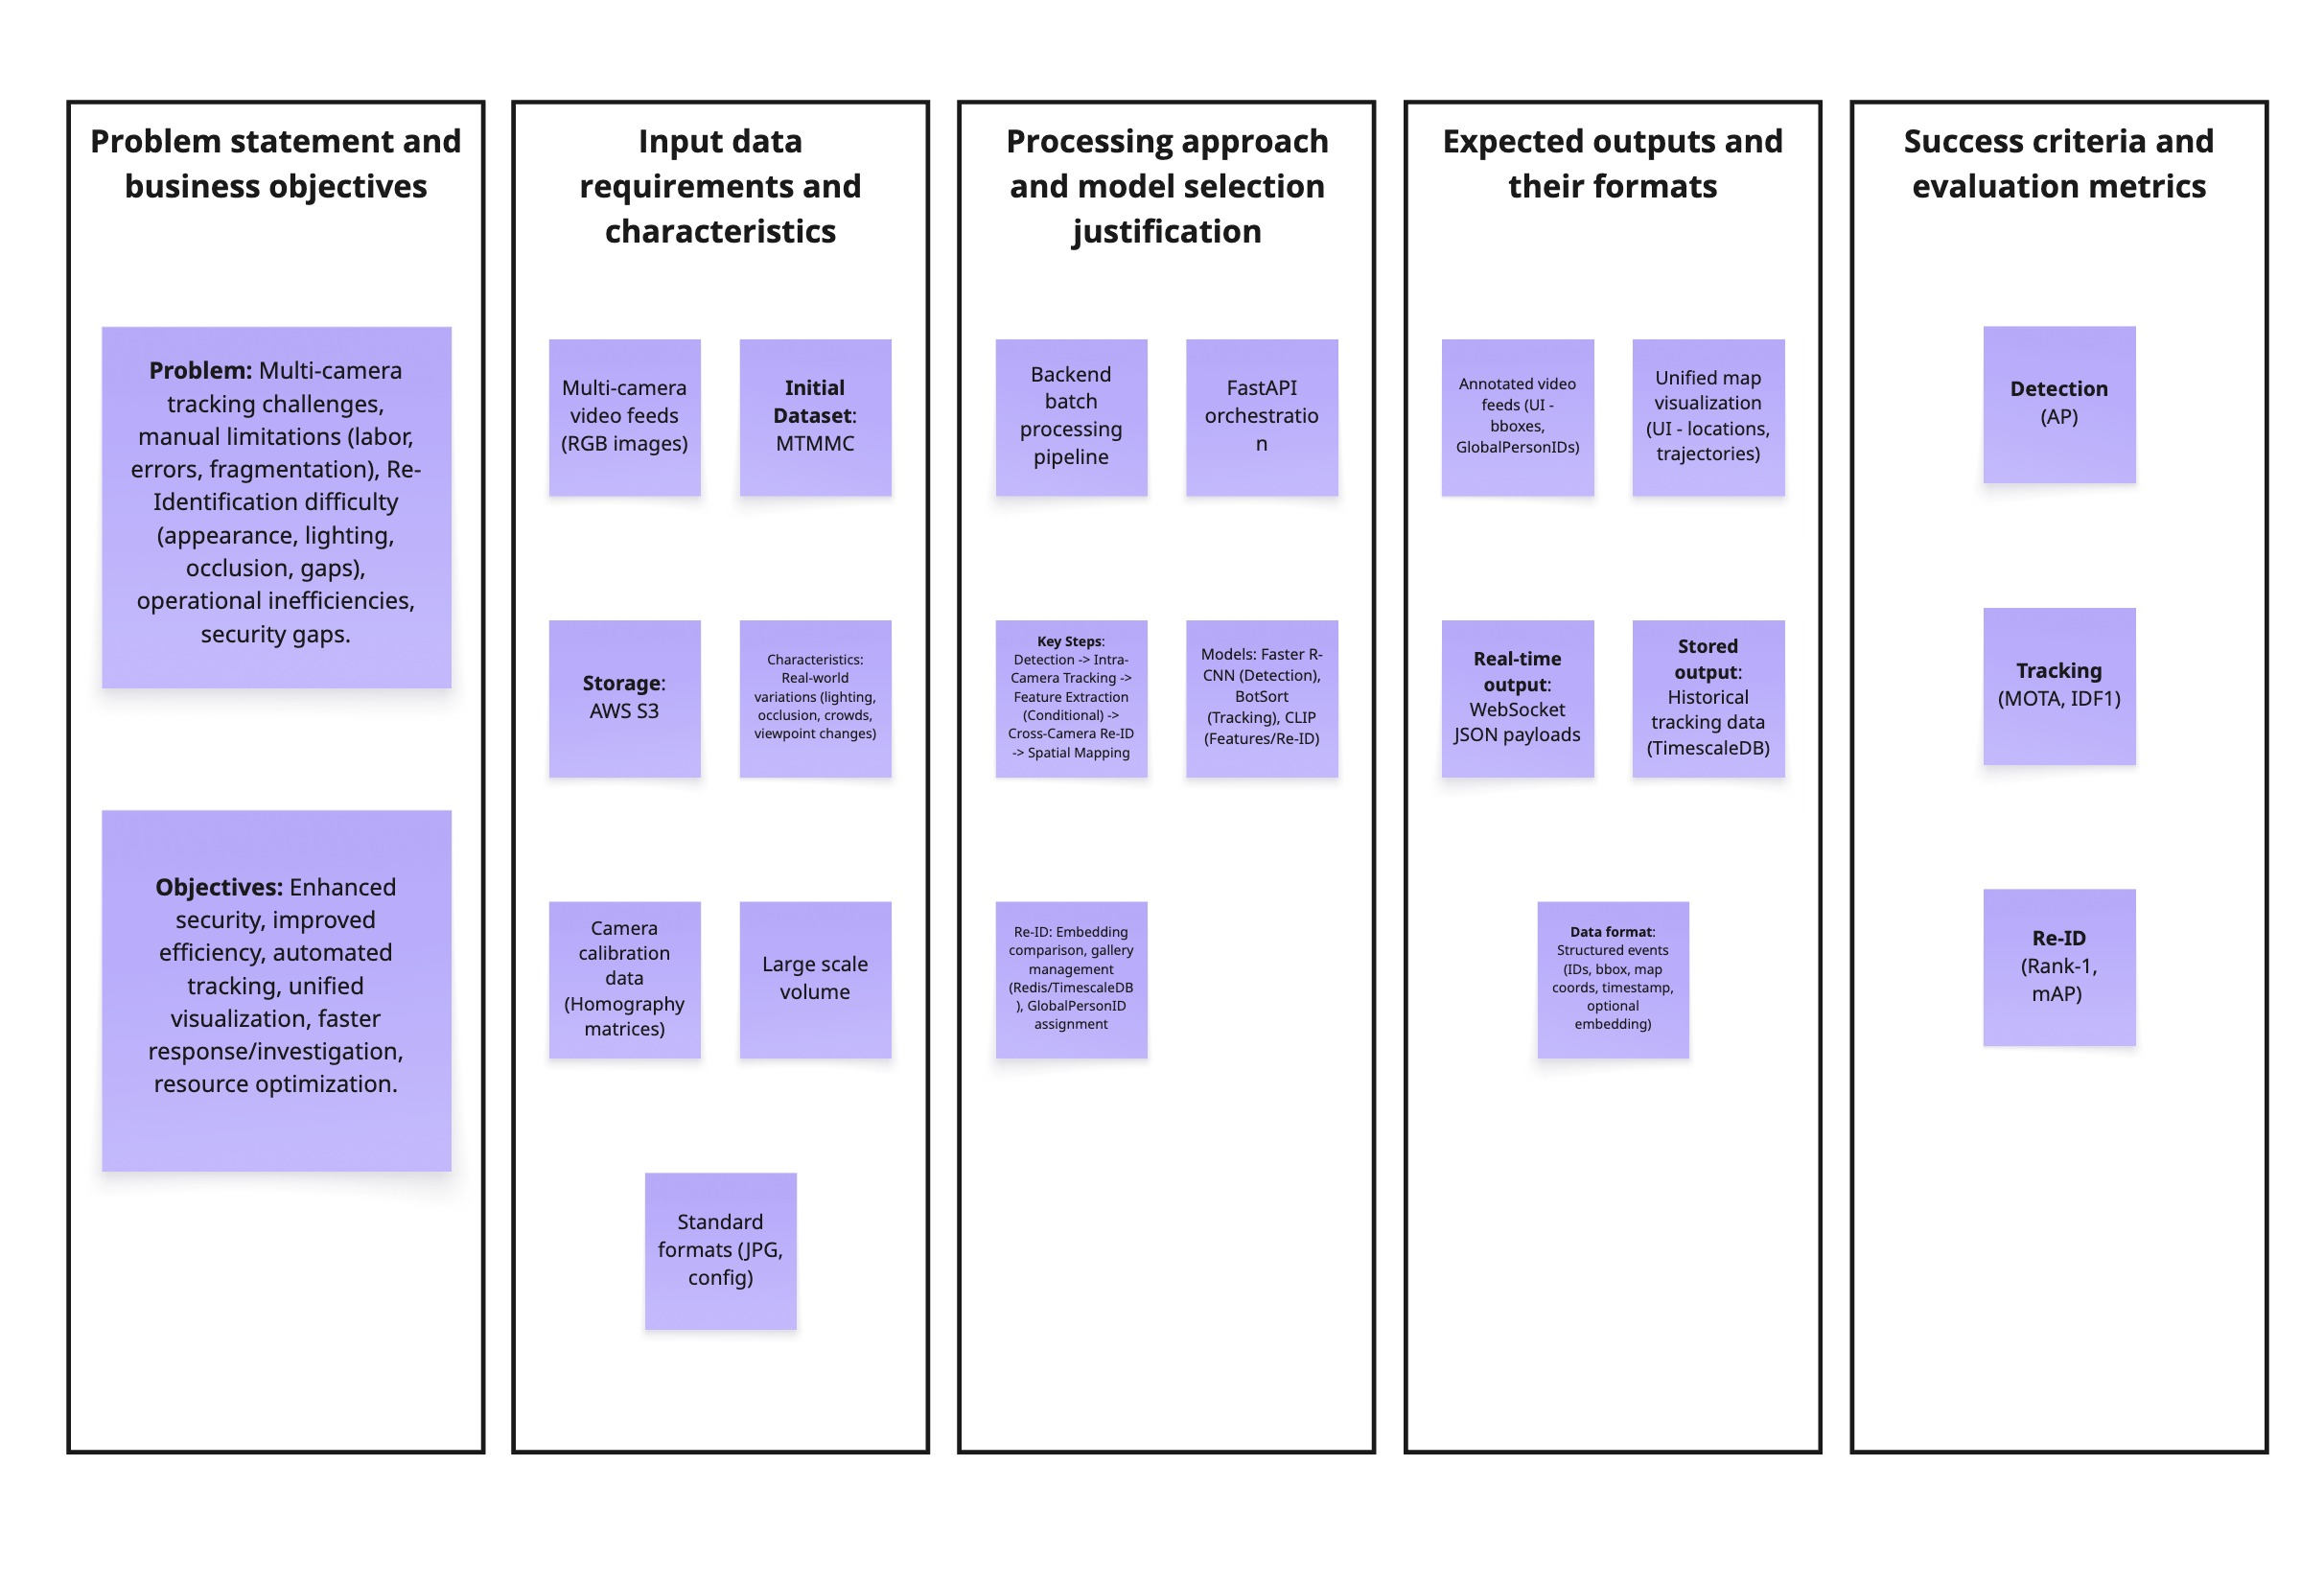
\includegraphics[width=1.0\textwidth, keepaspectratio]{jubjones/ml_canvas.jpg}
    }
    \caption{ML Canvas for Intelligent Multi-Camera Person Tracking and Analytics System}
    \label{fig:ml_canvas}
\end{figure}
\begin{itemize}
    \item \textbf{Problem Statement \& Business Objectives (ML Canvas):}
        The system directly addresses the significant challenges security and facility personnel face in tracking individuals across complex, multi-camera environments. It tackles the limitations of manual monitoring—its labor intensity, error propensity, and fragmented views—and the core technical hurdle of maintaining consistent identity (Re-Identification) despite variations in appearance, lighting, occlusions, and camera viewpoints. The overarching business objectives are to enhance safety, improve operational efficiency by automating tracking, provide unified spatial visualization of movement, reduce incident investigation time, and optimize resource allocation based on analytics.

    \item \textbf{Input Data Requirements (ML Canvas):}
        The necessary components for the system primarily involve recorded RGB video feeds or image sequences from multiple cameras, initially using datasets like MTMMC stored on AWS S3. These inputs encapsulate real-world challenges such as diverse lighting, occlusions, crowds, and viewpoint changes. Crucially, pre-calculated camera calibration data (Homography matrices) are also specified as essential inputs for spatial mapping. The large-scale data volume and standard formats (e.g., JPG, config files) are acknowledged requirements.

    \item \textbf{Processing Approach \& Model Selection (ML Canvas):}
        Central to the design is a backend-driven batch processing pipeline orchestrated by FastAPI. This pipeline integrates key AI steps in sequence:
        \begin{enumerate}[label=(\Alph*)]
            \item Person Detection, utilizing Faster R-CNN for robust object localization.
            \item Intra-Camera Tracking, employing algorithms like BotSort to maintain temporary IDs within single camera views.
            \item Conditional Feature Extraction for Re-ID, using CLIP to generate discriminative embeddings under specific triggers.
            \item Cross-Camera Re-Identification, which compares embeddings against a gallery (managed via Redis/TimescaleDB) to assign persistent GlobalPersonIDs.
            \item Spatial Mapping, applying the input homography matrices via OpenCV to project detected locations onto a unified map.
        \end{enumerate}
        The justifications for each model choice emphasize accuracy, robustness, and efficiency.

    \item \textbf{Expected Outputs (ML Canvas):}
        The system's outputs encompass both user-facing visualizations and stored data for analysis.
        \begin{itemize}
            \item \textit{For the UI:} Annotated video feeds displaying bounding boxes and GlobalPersonIDs, alongside a unified map interface showing current locations and historical paths. These are delivered via WebSocket JSON payloads.
            \item \textit{For historical analysis:} Structured tracking events (timestamp, IDs, coordinates, optional embeddings) stored in a TimescaleDB database.
        \end{itemize}

    \item \textbf{Success Criteria \& Evaluation Metrics (ML Canvas):}
        A dual approach to measuring performance is outlined:
        \begin{itemize}
            \item \textit{AI Model-Level Metrics (Offline Evaluation):} Specific metrics such as AP (Average Precision), MOTA (Multiple Object Tracking Accuracy), IDF1 (ID F1-Score), Rank-1 accuracy, and mAP (mean Average Precision) using dedicated test sets.
            \item \textit{System and Business-Level Metrics (Online/Operational Assessment):} Critical indicators including efficiency gains, reduction in incident investigation response time, user satisfaction levels, task completion rates for key scenarios, and overall system reliability.
        \end{itemize}
\end{itemize}
This detailed ML Canvas provides a comprehensive blueprint for the development and evaluation of this intelligent surveillance system, specifying the concrete choices and flows for the machine learning pipeline.


\subsection{Innovation}
\label{subsection:innovation}
While \usevar{\srsTitle} leverages established state-of-the-art AI techniques for tasks like detection, tracking, and re-identification, its core innovation lies in the effective integration and adaptation of these methods to address the specific, challenging problem of robust multi-camera person tracking in complex real-world environments. Many existing solutions excel at single-camera tracking but falter when attempting to maintain identity consistently across non-overlapping views with temporal gaps—precisely the gap \usevar{\srsTitle} aims to fill. The combination of accurate detection, persistent intra-camera tracking, discriminative Re-ID, and unified spatial mapping into a cohesive system designed for practical deployment represents a significant advancement tailored for campus and factory surveillance needs where multi-camera coverage is essential.


\section{AI Model Development, Training, and Evaluation}
\label{section:ai_model_dev_train_eval}

This section details the core AI model development lifecycle, including training procedures, fairness analysis, comparative experimentation for model selection, and methods for model interpretability.

\subsection{Model Training Implementation}
\label{subsection:model_training_impl}
This subsection details the implementation process for training the person detection model (Faster R-CNN) for the Intelligent Multi-Camera Person Tracking and Analytics System. The implementation utilizes PyTorch and TorchVision, leveraging pre-trained weights and fine-tuning on the MTMMC dataset. MLflow is used for tracking experiments and results.

\textbf{Basic Input Data Exploration \& Preprocessing Functions:}

\textit{Data Exploration:} An initial Exploratory Data Analysis (EDA) was performed (detailed separately, referencing src/pipelines/eda\_pipeline.py and configs/eda\_config.yaml). This explored aspects like dataset structure, frame counts per camera, annotation distributions (bounding box sizes, track lengths), and performed quality checks (missing GT, invalid annotations, frame count mismatches, out-of-bounds boxes, image dimension consistency). The provided EDA summary artifact confirms key preprocessing parameters.

\textit{Data Types \& Basic Statistics:}
\begin{itemize}
    \item Images are loaded as NumPy arrays (BGR format) using OpenCV (cv2.imdecode).
    \item Annotations are loaded from gt.txt files and initially processed as tuples (obj\_id, cx, cy, w, h).
    \item The EDA summary indicates original image dimensions are consistently 1920x1080 pixels in the sampled data.
\end{itemize}

\textit{Preprocessing Pipeline (src/data/training\_dataset.py, src/training/runner.py -> get\_transform):}
\begin{itemize}
    \item Loading: Images and annotations are loaded per frame per camera using MTMMCDetectionDataset.
    \item Color Conversion: Images are converted from BGR to RGB format suitable for TorchVision models.
    \item Resizing: Images are resized to a target input width (e.g., 640 pixels, as specified in configs/eda\_config.yaml and confirmed by the EDA summary artifact) while maintaining the aspect ratio. The EDA summary shows this results in resized dimensions of 640x360.
    \item ToTensor \& Scaling: Images are converted to PyTorch Tensors (torch.float32) and pixel values are scaled to the range [0.0, 1.0].
    \item Normalization: Standard ImageNet normalization is applied using mean [0.485, 0.456, 0.406] and standard deviation [0.229, 0.224, 0.225] (confirmed by EDA summary artifact).
    \item Augmentation (Training Only): Random horizontal flipping (p=0.5) is applied during training (get\_transform(train=True)).
    \item Target Formatting: Ground truth bounding boxes (cx, cy, w, h) are converted to the XYXY format ([xmin, ymin, xmax, ymax]) expected by Faster R-CNN. Labels are assigned (class ID 1 for 'person'). Both boxes and labels are wrapped in tv\_tensors (specifically tv\_tensors.BoundingBoxes) for compatibility with TorchVision's v2 transforms.
    \item Collation: A custom collate\_fn (src/utils/torch\_utils.py) is used by the DataLoader to handle batches, ensuring images are grouped as a list of tensors and targets remain a list of dictionaries.
\end{itemize}

\textbf{Model Architecture Definition:}

\textit{Model Choice:} The selected model is Faster R-CNN with a ResNet-50 backbone and Feature Pyramid Network (FPN), obtained from torchvision.models.detection.fasterrcnn\_resnet50\_fpn.

\textit{Architecture Overview:} Faster R-CNN is a two-stage object detector.
\begin{itemize}
    \item Stage 1 (Region Proposal Network - RPN): Scans the feature map (from ResNet-50 + FPN) to propose candidate regions (regions of interest - RoIs) that might contain objects.
    \item Stage 2 (RoI Head): Extracts features for each proposed RoI using RoIAlign and performs classification (object vs. background, or specific object classes) and bounding box regression to refine the box coordinates.
\end{itemize}

\textit{Pre-trained Weights:} The model is initialized using pre-trained weights from ImageNet (specifically FasterRCNN\_ResNet50\_FPN\_Weights.DEFAULT as specified in fasterrcnn\_training\_config.yaml).

\textit{Head Modification:} The pre-trained classification head (box predictor) is replaced with a new {FastRCNNPredictor} instance. This new head is configured for the specific number of classes required for this task: 2 (Person + Background), as defined in fasterrcnn\_training\_config.yaml.

\textit{Fine-tuning:} The number of trainable layers in the ResNet-50 backbone can be configured via trainable\_backbone\_layer (set to 3 in the config), allowing for fine-tuning deeper parts of the network.

\textbf{Training Loop \& Hyperparameters:}

\textit{Orchestration:} The training process is orchestrated by src/run\_training\_fasterrcnn.py, which loads the configuration (configs/fasterrcnn\_training\_config.yaml), sets up MLflow, and calls src/training/runner.py (run\_single\_training\_job).

\textit{Engine:} The core training and validation logic resides in the PyTorch engine (src/training/pytorch\_engine.py).

\textit{Hyperparameters (from configs/fasterrcnn\_training\_config.yaml}):
\begin{itemize}
    \item epochs: 5 (Note: This is low, indicative of a sample run).
    \item batch\_size: 2.
    \item optimizer: AdamW.
    \item learning\_rate: 0.001 (initial).
    \item weight\_decay: 0.005.
    \item lr\_scheduler: StepLR (decays LR by gamma=0.1 every step\_size=3 epochs).
    \item gradient\_clip\_norm: 1.0 (Max gradient norm for clipping).
\end{itemize}

\textit{Loss Calculation:} The standard Faster R-CNN loss components (RPN classification, RPN regression, RoI head classification, RoI head regression) are calculated internally by the TorchVision model during the forward pass. The {train\_one\_epoch} function sums these component losses for backpropagation.

\textit{Device:} Training runs on the device selected via the configuration ('auto', 'cuda', 'cpu', etc.), resolved using src/utils/device\_utils.py.

\textit{Mixed Precision:} Automatic Mixed Precision (AMP) is enabled via torch.cuda.amp.GradScaler when training on CUDA devices to potentially speed up training and reduce memory usage.

\textit{Checkpointing:} Model checkpoints (including model state, optimizer state, epoch, and validation metrics) are saved after each epoch. The best-performing checkpoint based on a specified validation metric (val\_map\_50 in the config) is also saved separately. Checkpoints are stored under a directory specified in the config (checkpoints), organized by run ID.

\textbf{Validation Methodology:}

\textit{Data Split:} The MTMMCDetectionDataset performs a random split of the loaded (and potentially subsetted) data into training and validation sets based on the val\_split\_ratio (0.2 or 20\% in the config).

\textit{Frequency:} Validation is performed at the end of each training epoch using the evaluate function in src/training/pytorch\_engine.py.

\textit{Metrics:}
\begin{itemize}
    \item Validation Loss: The average loss across all validation batches is calculated.
    \item Mean Average Precision (mAP): Standard COCO-style mAP metrics (mAP@[.5:.95], mAP@.50, mAP@.75) and Mean Average Recall (MAR) metrics are calculated using torchmetrics.detection.MeanAveragePrecision. The evaluation uses the configured person\_class\_id (1 for the PyTorch model) to identify relevant detections and ground truth.
\end{itemize}

\textbf{Results Analysis (Initial Sample Run):}

\textit{Disclaimer:} The following results are from an initial sample fine-tuning run. As specified in fasterrcnn\_training\_config.yaml, this run used only a fraction of the available data (use\_data\_subset: true, data\_subset\_fraction: 0.1) and ran for a limited number of epochs (epochs: 5). A full training process would require using the complete dataset, significantly more epochs, and potentially further hyperparameter optimization.

\begin{table}[!htb]
    \centering
    \caption{Initial Sample Run Results for Faster R-CNN Fine-tuning}
    \label{tab:fasterrcnn_sample_results}
    \begin{tabular}{@{}lc@{}}
        \toprule
        Metric                      & Value   \\ \midrule
        {eval\_map}           & 0.6522  \\
        {eval\_map\_50}        & 0.8954  \\
        {eval\_map\_75}        & 0.7522  \\
        {eval\_map\_small}     & 0.3798  \\
        {eval\_map\_medium}    & 0.6751  \\
        {eval\_map\_large}     & 0.8463  \\
        {eval\_mar\_1}         & 0.4318  \\
        {eval\_mar\_10}        & 0.7013  \\
        {eval\_mar\_100}       & 0.7088  \\
        {eval\_mar\_small}     & 0.4132  \\
        {eval\_mar\_medium}    & 0.7241  \\
        {eval\_mar\_large}     & 0.8730  \\
        {eval\_ap\_person}     & -1.0    \\
        {val\_loss\_classifier}& 0.0360  \\
        {val\_loss\_box\_reg}  & 0.1029  \\
        {val\_loss\_objectness}& 0.0417  \\
        {val\_loss\_rpn\_box\_reg}& 0.0472  \\
        {val\_total\_loss}     & 0.2278  \\
        {train\_total\_loss}   & 0.2260  \\ \bottomrule
    \end{tabular}
\end{table}

\textit{Interpretation (Preliminary):}
\begin{itemize}
    \item The overall mAP (0.6522) suggests the model learned effectively even on the small subset and few epochs.
    \item The high mAP@.50 (0.8954) indicates good performance at detecting persons with reasonable overlap, while the mAP@.75 (0.7522) shows decent localization accuracy.
    \item Training and validation losses (0.226 vs 0.228) are very close, suggesting no significant overfitting occurred during this short run on the data subset.
    \item The eval\_ap\_person metric is -1.0, indicating it wasn't successfully calculated or reported in this specific run. This could be due to various reasons, including potential misconfiguration in the metric calculation step for per-class AP, or insufficient examples of the 'person' class in the validation subset.
    \item These results are promising for a baseline but require comprehensive training on the full dataset for robust evaluation and deployment.
\end{itemize}

\textbf{Unit Testing:}
\textit{Purpose:} To validate key functionality within the training pipeline components, unit tests were implemented using pytest. These tests focus on isolating and verifying the behaviour of individual functions and classes.

\textit{Test Structure:} Tests are organized within the tests/ directory, mirroring the src/ structure (e.g., tests/data, tests/evaluation, tests/training, tests/utils). pytest fixtures defined in tests/conftest.py (e.g., mock\_fasterrcnn\_config, cpu\_device, mock\_project\_root) provide standardized mock data and configurations for the tests.

\textit{Key Areas Tested:}
\begin{itemize}
    \item Dataset (tests/data/test\_training\_dataset.py):
    \begin{itemize}
        \item Verifies the MTMMCDetectionDataset's \_\_getitem\_\_ method correctly loads image data and formats annotations (including empty annotations) into the required tv\_tensors structure (e.g., BoundingBoxes in XYXY format).
        \item Uses mocking (unittest.mock.patch) to isolate the dataset class from actual file system reads (Path.is\_file, np.fromfile, cv2.imdecode) and the initial data loading scan (\_load\_data\_samples).
        \item Tests the get\_transform utility function to ensure correct transforms are applied for training vs. validation modes.
    \end{itemize}
    \item Metrics (tests/evaluation/test\_metrics.py):
    \begin{itemize}
        \item Validates the interface and basic flow of the compute\_map\_metrics function.
        \item Mocks the torchmetrics.detection.MeanAveragePrecision class to simulate metric calculation without requiring the actual library or extensive data.
        \item Asserts that the update and compute methods of the mocked metric object are called correctly and that the results dictionary has the expected structure.
        \item Tests are skipped (pytest.mark.skipif) if torchmetrics is not installed.
    \end{itemize}
    \item Training Runner (tests/training/test\_runner.py):
    \begin{itemize}
        \item Tests the get\_fasterrcnn\_model function responsible for loading the Faster R-CNN model.
        \item Mocks the underlying torchvision.models.detection.fasterrcnn\_resnet50\_fpn function and weights enum to ensure the correct pre-trained weights and trainable\_backbone\_layers are requested.
        \item Verifies that the model's classification head (box predictor) is replaced, a key step in fine-tuning.
    \end{itemize}
    \item Utilities (tests/utils/test\_torch\_utils.py):
    \begin{itemize}
        \item Tests the collate\_fn to ensure it correctly batches image tensors and target dictionaries, including handling empty targets.
        \item Tests the get\_optimizer factory function to confirm it returns the correct optimizer instances (e.g., AdamW, SGD) based on the name provided.
        \item Tests the get\_lr\_scheduler factory function to verify it returns the appropriate scheduler instances (e.g., StepLR, CosineAnnealingLR) or None for unsupported names.
    \end{itemize}
\end{itemize}

\subsection{Model Fairness Analysis}
\label{subsection:model_fairness_analysis}
Ensuring fairness in AI systems is critical, especially in security and surveillance applications where biases can lead to disproportionately negative outcomes for certain groups. While a full quantitative fairness audit requires specific demographic ground truth data often unavailable in datasets like MTMMC, we can analyze potential biases and discuss mitigation strategies relevant to the Intelligent Multi-Camera Person Tracking and Analytics System.

\textbf{1. Potential Sources of Bias in Training Data (MTMMC Dataset)}
The MTMMC dataset, while valuable for its scale and real-world complexity, may contain inherent biases that could influence model performance:
\begin{itemize}
    \item Demographic Imbalance:
    \begin{itemize}
        \item \textit{Geographic/Ethnic Bias:} Collected at a specific campus (KAIST) and factory in Korea, the dataset likely features a population predominantly of East Asian descent. Models trained on this data might exhibit lower performance (e.g., lower detection recall or Re-ID accuracy) for individuals from underrepresented ethnicities or races.
        \item \textit{Age/Gender Bias:} The distribution of age groups and genders within the campus/factory setting might not reflect broader population distributions. If certain groups are less frequent, the model may learn less robust features for them.
        \item \textit{Clothing Style Bias:} Campus environments often have common clothing styles (e.g., student attire). The model might struggle with less common or culturally specific attire not well-represented in the training data, potentially impacting Re-ID.
    \end{itemize}
    \item Environmental \& Situational Bias:
    \begin{itemize}
        \item \textit{Lighting Conditions:} While diverse, if certain lighting conditions (e.g., very low light, harsh shadows, specific times of day) are underrepresented compared to well-lit scenarios, the detection and Re-ID models might perform unfairly worse under those specific conditions.
        \item \textit{Camera Viewpoint/Quality:} Some camera views might be inherently more challenging (e.g., distant, oblique angles, lower resolution feeds). Individuals primarily observed through these cameras might be tracked less reliably. The system's performance might be less "fair" to individuals who happen to frequent areas covered only by poor-quality views.
        \item \textit{Occlusion Levels:} Individuals frequently moving through crowded areas or behind obstacles will experience higher occlusion rates. If the training data doesn't sufficiently cover heavy occlusion scenarios, the tracking (MOTA/IDF1) and Re-ID might unfairly penalize people in dense environments.
        \item \textit{Behavioral Patterns:} The dataset likely captures typical pedestrian movements. Individuals with atypical gaits or movement patterns might be tracked less effectively.
    \end{itemize}
    \item Annotation Bias:
    \begin{itemize}
        \item \textit{Labeling Errors/Omissions:} Manual or semi-automated annotation processes might be prone to errors. Annotators might be less likely to accurately label individuals who are distant, heavily occluded, or appear briefly, potentially leading to biases against detecting or tracking such individuals.
    \end{itemize}
\end{itemize}

\textbf{2. Fairness Metric Calculation (Conceptual Implementation)}
Directly calculating fairness metrics like Equal Opportunity or Demographic Parity requires ground truth sensitive attributes (e.g., ethnicity, gender) linked to person IDs, which are not typically part of the MTMMC annotations. However, we can use proxy analyses by evaluating performance disparities across groups defined by observable characteristics or conditions:
\begin{itemize}
    \item Metric: Re-Identification Accuracy Disparity (e.g., Rank-1 Accuracy or mAP difference).
    \item Groups: Define groups based on conditions where bias is suspected. Examples:
    \begin{enumerate}
        \item Group A: Tracks primarily observed in well-lit conditions (e.g., average pixel intensity > threshold).
        \item Group B: Tracks primarily observed in low-lit conditions (e.g., average pixel intensity < threshold).
        OR
        \item Group C: Tracks with low average occlusion (< 20\% bounding box occlusion across frames).
        \item Group D: Tracks with high average occlusion (> 50\% bounding box occlusion across frames).
        OR
        \item Group E: Tracks where the person's bounding box size is consistently large (e.g., average height > 100 pixels).
        \item Group F: Tracks where the person's bounding box size is consistently small (e.g., average height < 50 pixels).
    \end{enumerate}
    \item Calculation Steps:
    \begin{enumerate}
        \item Identify and isolate tracklets belonging to each group within the MTMMC test set based on frame metadata or derived properties (lighting, occlusion estimates, bbox size).
        \item Run the Re-ID component (e.g., CLIP feature extraction + gallery matching) on the test queries corresponding to each group.
        \item Calculate Rank-1 Accuracy (or mAP) separately for Group A vs. Group B, Group C vs. Group D, etc.
        \item Fairness Assessment: Compare the metrics. A significant drop in performance for one group (e.g., Rank-1 accuracy is 85\% for Group E but only 60\% for Group F) indicates a fairness issue related to that characteristic (distance/size in this case). The fairness metric could be the difference (e.g., 25\% drop) or ratio (e.g., 0.71) of the scores.
    \end{enumerate}
\end{itemize}

\textbf{3. Approaches to Mitigate Detected Bias}
If fairness analysis reveals significant performance disparities, several strategies can be employed:
\begin{itemize}
    \item Data-Based Mitigation:
    \begin{itemize}
        \item \textit{Targeted Data Augmentation:} Intensify augmentations simulating the conditions where the model underperforms (e.g., synthesize more low-light variations, add artificial occluders, use style transfer to diversify clothing appearances).
        \item \textit{Data Balancing/Re-sampling:} If demographic labels become available or reliable proxies are found, use techniques like over-sampling underrepresented groups or under-sampling overrepresented groups during training. Generate synthetic data (if feasible) for minority groups.
        \item \textit{Curriculum Learning:} Structure the training process to initially focus on easier examples and gradually introduce more challenging or underrepresented scenarios.
    \end{itemize}
    \item Model-Based Mitigation:
    \begin{itemize}
        \item \textit{Adversarial Debiasing:} If sensitive attributes are known, train the feature extractor (e.g., CLIP) with an additional adversarial loss that discourages the model from encoding information about the sensitive attribute, aiming for representations invariant to that attribute.
        \item \textit{Fairness Regularization:} Add terms to the model's loss function that explicitly penalize performance disparities between defined groups (requires group labels).
        \item \textit{Domain Generalization:} Employ techniques specifically designed to improve model robustness across different domains (e.g., varying lighting, camera types), which can indirectly improve fairness by reducing performance gaps caused by environmental variations.
    \end{itemize}
    \item Post-processing Mitigation:
    \begin{itemize}
        \item \textit{Group-Specific Thresholds:} Carefully adjust decision thresholds (e.g., Re-ID similarity score threshold) for different groups or conditions identified as problematic.
    \end{itemize}
    \item Operational Mitigation:
    \begin{itemize}
        \item \textit{Transparency \& User Training:} Make users aware of the system's limitations and potential biases (e.g., "Performance may be lower in dimly lit areas"). Train operators to critically evaluate the system's output, especially in challenging conditions.
        \item \textit{Feedback Mechanism:} Allow users to easily flag incorrect identifications or tracking failures. This feedback can be invaluable for identifying systematic biases and informing targeted retraining efforts.
        \item \textit{Continuous Monitoring:} Regularly re-evaluate fairness metrics on updated datasets or newly collected operational data to track bias drift and ensure mitigation strategies remain effective.
    \end{itemize}
\end{itemize}
By proactively considering these potential biases and incorporating fairness analysis and mitigation strategies, we aim to develop a more equitable and trustworthy multi-camera tracking system.

\subsection{Model Selection via Experimentation}
\label{subsection:model_selection_experimentation}
To select the optimal person detection model for the Intelligent Multi-Camera Person Tracking and Analytics System, several candidate architectures were evaluated using MLflow for experiment tracking and comparison. This allows for systematic tracking of model parameters, configurations, and performance metrics across different runs.

\textbf{Experiment Setup:}
We compared four distinct person detection models representing different architectural approaches:
\begin{itemize}
    \item Faster R-CNN (fasterrcnn\_resnet50): A representative Two-Stage CNN detector, known for high accuracy, particularly with varying object sizes.
    \item RT-DETR (rtdetr\_x): A Vision Transformer (ViT) based detector, often achieving a good balance between speed and accuracy.
    \item RT-DETR (rtdetr\_l): Another variant of the RT-DETR model.
    \item YOLO (yolo11x): A representative One-Stage CNN detector, typically prioritized for speed.
\end{itemize}
Using the MLflow Tracking UI (as illustrated conceptually in Figures \ref{fig:mlflow_comparison_1} and \ref{fig:mlflow_comparison_2}), we logged key parameters for each run, including:
\begin{itemize}
    \item model.model\_name: Specific identifier for the model variant (e.g., fasterrcnn\_resnet50, rtdetr\_x).
    \item model.type: The general architecture type (e.g., fasterrcnn, rtdetr, yolo).
    \item model.weights\_path: Path to the pre-trained weights used for the specific experiment.
    \item model.person\_class\_id: The class ID designated for 'person' detections within the model's output.
\end{itemize}

\begin{figure}[!htb]
    \centering
    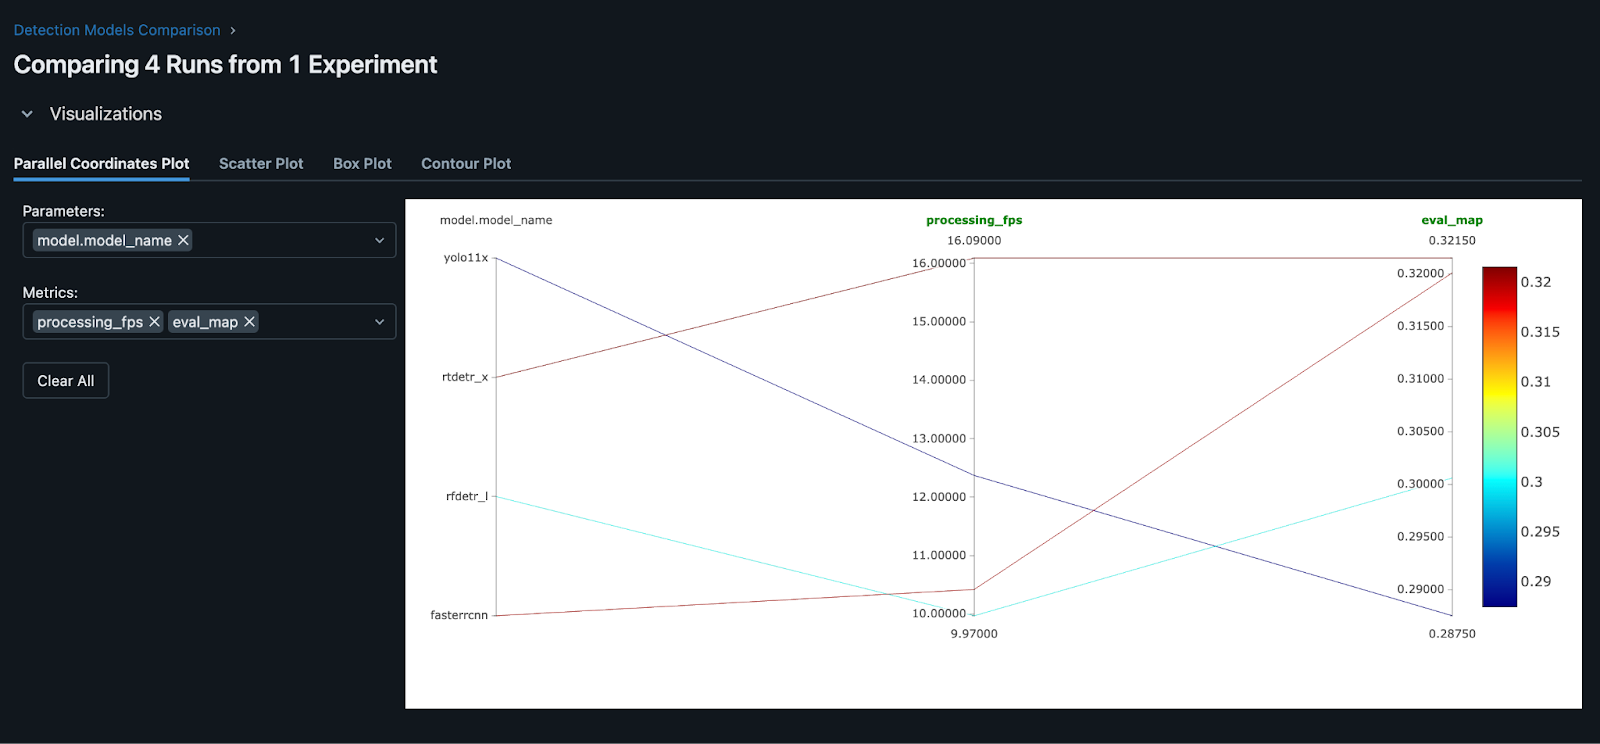
\includegraphics[width=1.0\textwidth,keepaspectratio]{jubjones/mlflow_comparison_1.png} % Placeholder
    \caption{Conceptual MLflow UI: Performance Metrics Chart}
    \label{fig:mlflow_comparison_1}
\end{figure}

\begin{figure}[!htb]
    \centering
    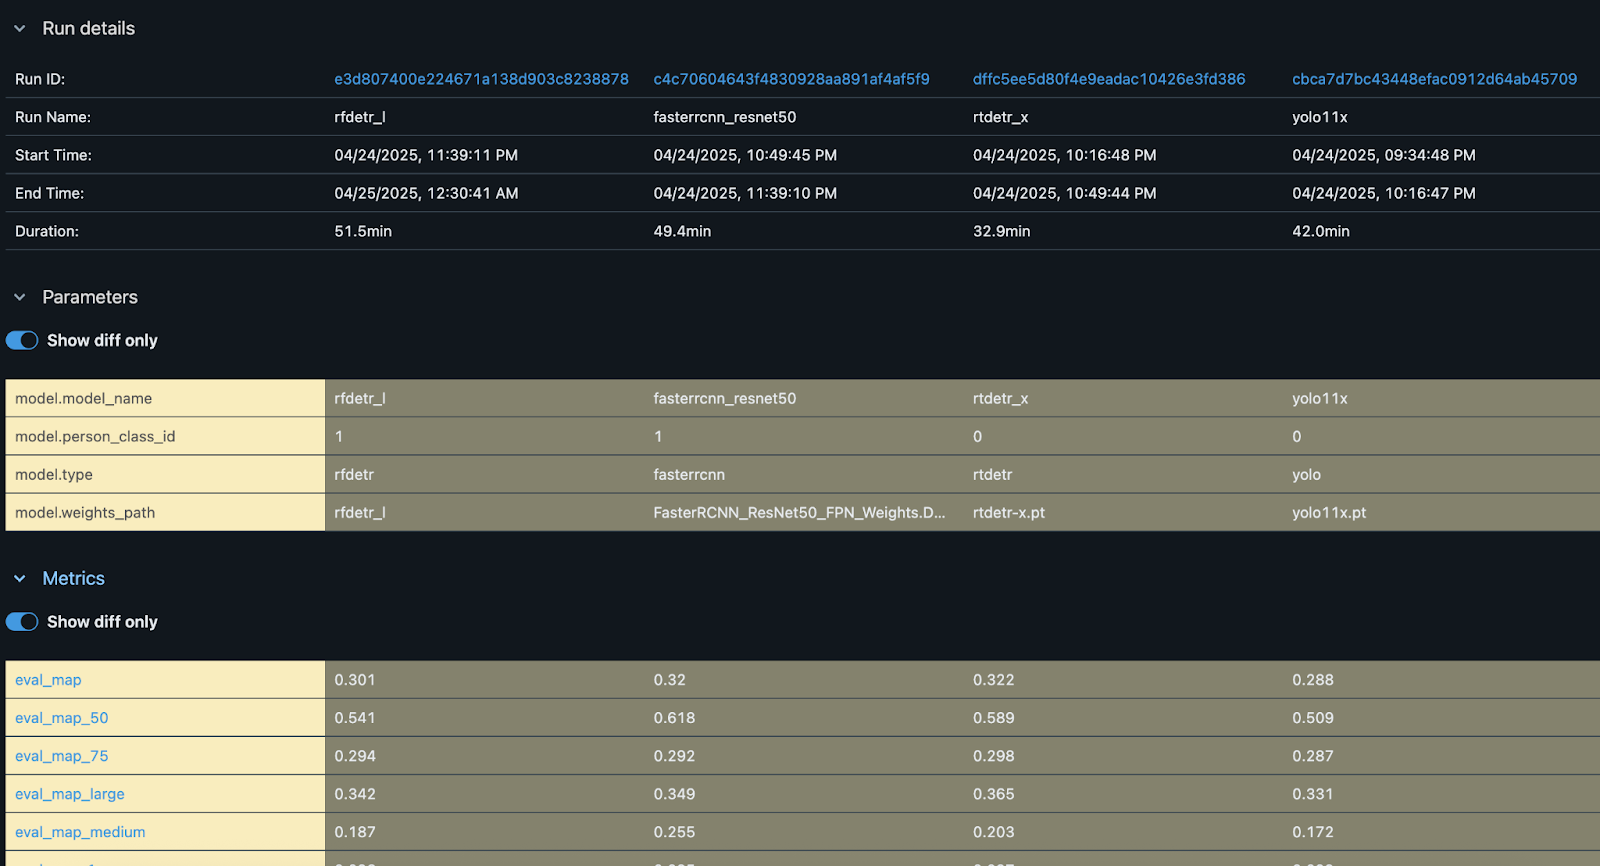
\includegraphics[width=1.0\textwidth,keepaspectratio]{jubjones/mlflow_comparison_2.png} % Placeholder
    \caption{Conceptual MLflow UI: The table summarizes key performance metrics extracted from the MLflow comparison}
    \label{fig:mlflow_comparison_2}
\end{figure}
\clearpage

\textbf{Performance Comparison (Quantitative):}
The following table summarizes key performance metrics extracted from the MLflow comparison for the person detection task on the evaluation dataset:

\begin{table}[!htb]
  \centering
  \caption{Performance Comparison of Person Detection Models}
  \label{tab:model_performance_comparison}
  \resizebox{\textwidth}{!}{%
  \begin{tabular}{@{}lccccccccc@{}}
    \toprule
    Model Name & {eval\_ap\_person} & {eval\_map} & {eval\_map\_50} & {eval\_map\_75} & {eval\_map\_large} & {eval\_map\_medium} & {eval\_map\_small} & {processing\_fps} & {total\_person\_detections} \\ \midrule
    {rtdetr\_x} & 0.322 & 0.322 & 0.497 & 0.334 & 0.496 & 0.203 & 0.039 & 16.09 & 156,107 \\
    {fasterrcnn\_resnet50} & 0.320 & 0.320 & 0.546 & 0.310 & 0.473 & 0.255 & 0.033 & 10.42 & 190,884 \\
    {rtdetr\_l} & 0.316 & 0.316 & 0.486 & 0.329 & 0.489 & 0.197 & 0.038 & 9.48 & 152,317 \\
    {yolo11x} & 0.297 & 0.297 & 0.481 & 0.295 & 0.453 & 0.188 & 0.030 & 11.66 & 110,645 \\ \bottomrule
  \end{tabular}%
  }
  \par\medskip\footnotesize
  Note: {eval\_ap\_person} represents the mean Average Precision specifically for the 'person' class, serving as our primary accuracy metric. Metrics like {eval\_map\_50}, {\_large}, {\_medium} provide insight into performance at different IoU thresholds and object sizes. {processing\_fps} measures inference speed, and {total\_person\_detections} indicates the raw count of detected persons.
\end{table}

\textbf{Key Observations:}
\begin{itemize}
    \item Overall Accuracy (mAP): RTDETR-X achieves the highest overall mAP (0.322), marginally beating Faster R-CNN (0.320). YOLO performs the lowest.
    \item Accuracy by Size: Faster R-CNN shows significantly better performance on medium-sized objects (mAP Medium): 0.255 vs. 0.203 for RTDETR-X). RTDETR-X has a slight edge on large objects. (Small object performance is not directly comparable from the AP metrics shown, but MAR metrics suggest similar performance at the top-1 recall level).
    \item Recall/Total Detections: Faster R-CNN detects considerably more persons overall (190,884) compared to RTDETR-X (156,107) and others. This suggests potentially better recall, crucial for not missing individuals in a tracking scenario.
    \item Speed (FPS): RTDETR-X is the fastest model (16.09 FPS), followed by YOLO, then Faster R-CNN and RTDETR-L.
\end{itemize}

\textbf{Justification for Final Model Selection (Baseline):}
Based on the quantitative comparison and qualitative observations during initial testing, Faster R-CNN (fasterrcnn\_resnet50) is selected as the baseline person detection model for the system. The justification is as follows:
\begin{enumerate}
    \item Superior Medium Object Performance: While RTDETR-X has the highest overall mAP, Faster R-CNN's significantly better performance on medium-sized objects (\ {eval\_map\_medium}) is critical in real-world surveillance where individuals are often not very close (large) or extremely far (small).
    \item Higher Detection Count (Recall): The substantially higher {total\_person\_detections} for Faster R-CNN strongly suggests better recall. In a tracking system, minimizing missed detections (false negatives) is often more critical than achieving the absolute highest precision, as a missed detection breaks the track entirely. This higher count likely reflects better performance on harder-to-detect individuals (potentially smaller, partially occluded).
    \item Qualitative Stability (NMS Issue): During practical application tests on the dataset videos, the RTDETR models were observed to occasionally suffer from Non-Maximal Suppression (NMS) issues, leading to multiple bounding boxes being predicted for the same person (over-prediction). While potentially tunable, this instability makes Faster R-CNN a more reliable starting point.
    \item Acceptable Speed: Although not the fastest, Faster R-CNN's processing speed (10.42 FPS) is deemed acceptable for the backend batch processing pipeline envisioned in the ML Canvas.
\end{enumerate}
Therefore, despite RTDETR-X showing marginally higher overall mAP and better speed, Faster R-CNN's robustness, particularly its strength in detecting medium-sized objects and its higher overall detection count (indicating better recall), combined with observed stability advantages, make it the preferred choice for the initial implementation. Further fine-tuning and comparison, potentially including a re-trained RTDETR addressing the NMS concerns, will be conducted in subsequent development phases.

\subsection{Model Explainability}
\label{subsection:model_explainability}
Understanding *how* the selected Faster R-CNN model arrives at its predictions is crucial for building trust and diagnosing potential issues. This task focuses on implementing and demonstrating techniques to interpret the model's internal workings, specifically identifying which parts of an input image influenced a particular detection.

\textbf{Methodology:}
\begin{itemize}
    \item   \textbf{Model:} Faster R-CNN (ResNet-50 + FPN backbone).
    \item   \textbf{Technique:} Gradient-weighted Class Activation Mapping (Grad-CAM) was chosen as the explainability method. Grad-CAM is suitable for CNN-based models like Faster R-CNN as it produces visual heatmaps highlighting the image regions most important for a specific output class score. We utilize the {LayerGradCam} implementation from the {captum} library.
    \item   \textbf{Configuration:} The process is configured via configs/explainability\_config.yaml, specifying the method ("gradcam"), the convolutional layer to target ({target\_layer\_name}, e.g., "backbone.body.layer4"), the confidence threshold to explain detections, and the class index for person (1).
    \item   \textbf{Code:} The core logic is implemented in {src/explainability/faster\_rcnn\_explainer.py} ({explain\_detection\_gradcam}), visualization in {src/explainability/visualization.py} ({visualize\_explanation}), and orchestrated by {src/run\_explainability.py}.
\end{itemize}

\textbf{Implementation Details:}
\begin{enumerate}
    \item  \textbf{Model \& Target Layer:} The pre-trained and fine-tuned Faster R-CNN model is loaded ({src/inference/detector.py -> load\_trained\_fasterrcnn}). The specified target layer (e.g., the last layer of the ResNet backbone body) is retrieved.
    \item  \textbf{Forward Function Wrapper:} A custom forward function is defined for Captum. This function takes the input image tensor, performs inference with the Faster R-CNN model, and specifically extracts the classification score for the target detection (identified by its index in the output list) and the target class ('person').
    \item  \textbf{Attribution Calculation:} {LayerGradCam} uses the model, the target layer, and the forward wrapper. Its {attribute} method is called with the input image tensor. It calculates the gradients of the target score with respect to the target layer's feature maps, weights these maps by the gradients, and produces a raw attribution heatmap.
    \item  \textbf{Visualization:} The raw heatmap is processed (summed across channels if necessary, normalized) and overlaid onto the original input image using OpenCV functions ({overlay\_heatmap}). Detected bounding boxes are drawn on the overlay, and the final visualization is saved as a PNG image.
\end{enumerate}

\textbf{Demonstration \& Results:}
The {run\_explainability.py} script executes this process on the images specified in the configuration. Below are examples from the run output, showing the generated visualizations for the top-scoring 'person' detection in each test image:

\begin{figure}[!htb]
    \centering
    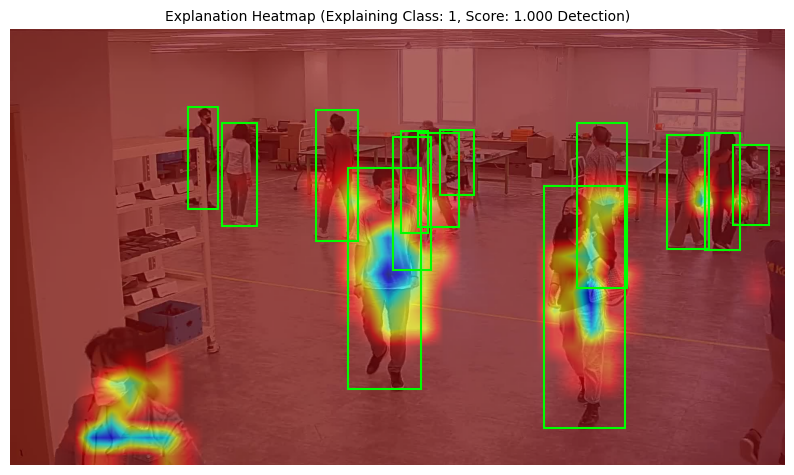
\includegraphics[width=1.0\textwidth,keepaspectratio]{jubjones/s10_c09_000000_explain_gradcam_det1_score1.00.png}
    \caption{Grad-CAM for Factory Scene (s10/c09/000000.jpg, Detection 1, Score: 0.9996)}
    \label{fig:gradcam_example1}
    \parbox{0.9\textwidth}{\footnotesize \textit{Interpretation:} The heatmap strongly highlights the torso and upper leg regions of the person within the bounding box. This focused activation pattern indicates that features in these areas were highly influential in the model's decision to classify this region as 'person' with extremely high confidence. The heatmap aligns well with the subject's silhouette.}
\end{figure}

\begin{figure}[!htb]
    \centering
    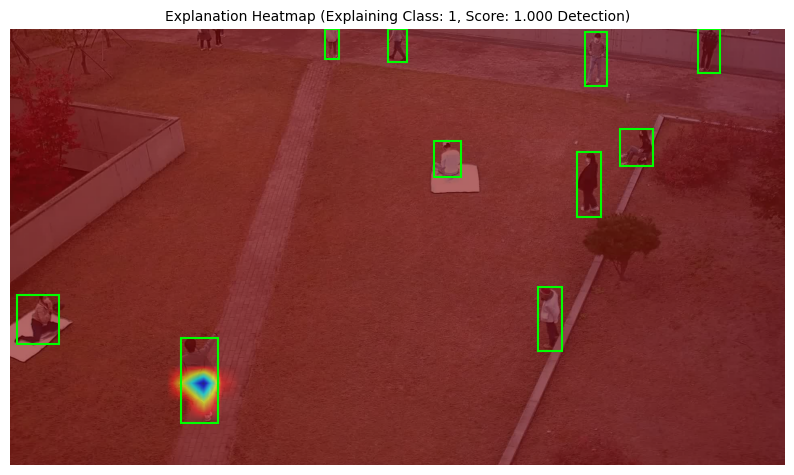
\includegraphics[width=1.0\textwidth,keepaspectratio]{jubjones/s47_c02_000000_explain_gradcam_det1_score1.00.png}
    \caption{Grad-CAM for Campus Scene (s47/c02/000000.jpg, Detection 1, Score: 0.9997)}
    \label{fig:gradcam_example2}
    \parbox{0.9\textwidth}{\footnotesize \textit{Interpretation:} For this smaller, more distant person, the Grad-CAM heatmap concentrates primarily on the upper body and head region. Even though the person occupies fewer pixels, the model clearly identifies relevant features, again correlating with the very high confidence score.}
\end{figure}

\begin{figure}[!htb]
    \centering
    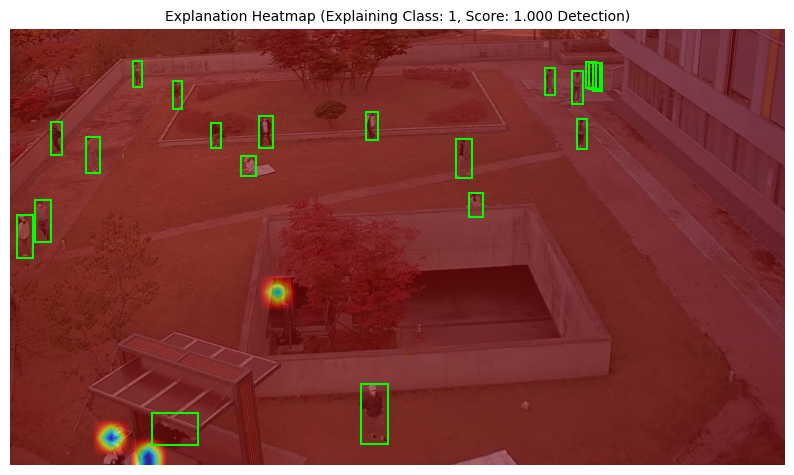
\includegraphics[width=1.0\textwidth,keepaspectratio]{jubjones/s47_c03_000000_explain_gradcam_det1_score1.00.png}
    \caption{Grad-CAM for Campus Scene (s47/c03/000000.jpg, Detection 1, Score: 0.9998)}
    \label{fig:gradcam_example3}
    \parbox{0.9\textwidth}{\footnotesize \textit{Interpretation:} Similar to Example 2, the heatmap focuses on the core body (torso) of the detected person. The activation is relatively contained within the person's boundaries, contributing to the high prediction score.}
\end{figure}
\clearpage
These visualizations provide valuable insights into the model's decision-making process, confirming that it generally focuses on relevant body parts for person detection. They serve as a tool for verifying expected behavior and potentially debugging cases where the model might focus on irrelevant background features or fail unexpectedly.

\subsection{Prediction Reasoning}
\label{subsection:prediction_reasoning}
Beyond visualizing where the model looks (Section \ref{subsection:model_explainability}), this task focuses on providing a human-understandable reason or justification for individual predictions made by the Faster R-CNN model.

\textbf{Mechanism Design:}
A mechanism was designed to generate textual reasoning based on the quantitative output of the model (confidence score) and the qualitative evidence from the explainability analysis (the existence of a Grad-CAM visualization).
\begin{itemize}
    \item   \textbf{Input:} Takes the detection result dictionary (containing 'box', 'label', 'score') and context (explanation type, visualization availability).
    \item   \textbf{Processing:} Uses heuristic rules based on the confidence score to infer the model's certainty (high, moderate, low). It explicitly mentions the confidence value and connects it to the presence or absence of strong visual features learned by the model. If a visual explanation (like Grad-CAM) was generated, the reasoning text refers the user to it for further insight into the influential image regions.
    \item   \textbf{Output:} Produces a textual string summarizing the reasoning for that specific prediction.
    \item   \textbf{Code:} The core logic is implemented in {src/explainability/reasoning.py} ({generate\_reasoning\_text}), and the overall process of applying it to detections and logging the results is handled in {src/run\_explainability.py} ({execute\_explainability}).
\end{itemize}

\textbf{Implementation Details:}
The {generate\_reasoning\_text} function constructs sentences based on the input detection's confidence score. It provides different qualitative interpretations for high (>= 0.9), moderate (>= 0.7), and lower confidence scores. It then appends a sentence directing the user to the generated visualization (if {has\_visualization} is True), mentioning the explanation type (e.g., "GRADCAM Focus") and the bounding box coordinates, encouraging review of the highlighted regions (e.g., head, torso). The {execute\_explainability} function iterates through the top detections for each configured input image, calls this reasoning function, and logs the output both to the console and aggregates it into a final summary file ({\_reasoning\_log.txt}).

\textbf{Example Outputs:}
The {run\_explainability.py} script was executed using the configuration {configs/explainability\_config.yaml} on the three specified test images. The following are the exact textual reasoning outputs generated for the same top-scoring detections analyzed visually in Section \ref{subsection:model_explainability}:

\textit{For s10/c09/000000.jpg (Detection 1, Score: 0.9996):}

Reasoning: Detected object classified as 'person' (label 1) with a 
confidence score of 1.00. This high confidence suggests the model 
found strong visual evidence matching features learned for the 
'person' class. The associated visualization (GRADCAM Focus) 
highlights the specific image regions that most influenced this 
classification decision. These influential regions are located 
primarily within the detected bounding box [523, 233, 611, 488]. 
Reviewing the heatmap overlay can provide further insight into which 
parts of the object (e.g., head, torso) contributed most to the 
prediction.


\textit{For s47/c02/000000.jpg (Detection 1, Score: 0.9997):}

Reasoning: Detected object classified as 'person' (label 1) with a 
confidence score of 1.00. This high confidence suggests the model 
found strong visual evidence matching features learned for the 
'person' class. The associated visualization (GRADCAM Focus) 
highlights the specific image regions that most influenced this 
classification decision. These influential regions are located 
primarily within the detected bounding box [1509, 248, 1592, 339]. 
Reviewing the heatmap overlay can provide further insight into which 
parts of the object (e.g., head, torso) contributed most to the 
prediction.

\textit{For s47/c03/000000.jpg (Detection 1, Score: 0.9998):}

Reasoning: Detected object classified as 'person' (label 1) with a 
confidence score of 1.00. This high confidence suggests the model 
found strong visual evidence matching features learned for the 
'person' class. The associated visualization (GRADCAM Focus) 
highlights the specific image regions that most influenced this 
classification decision. These influential regions are located 
primarily within the detected bounding box [617, 216, 651, 293]. 
Reviewing the heatmap overlay can provide further insight into which 
parts of the object (e.g., head, torso) contributed most to the 
prediction.

\textbf{Evaluation:}
The implemented mechanism successfully generates human-readable explanations for individual predictions. While not employing complex methods like SHAP (which can be challenging for object detectors), it fulfills the requirement by:
\begin{enumerate}
    \item  Interpreting the primary quantitative output (confidence score).
    \item  Relating the score to the model's perceived evidence strength.
    \item  Integrating the output of the explainability method (Grad-CAM) by directing the user to the visual evidence.
\end{enumerate}
This provides a practical level of reasoning suitable for understanding the basis of individual detection decisions within the system. The complete reasoning log for all explained detections across the test images is saved as an artifact ({outputs/explanations/*\_reasoning\_log.txt}).


\section{User Experience Design with AI}
\label{section:ux_design} % Kept original unique label

\begin{figure}[H]
    \centering
    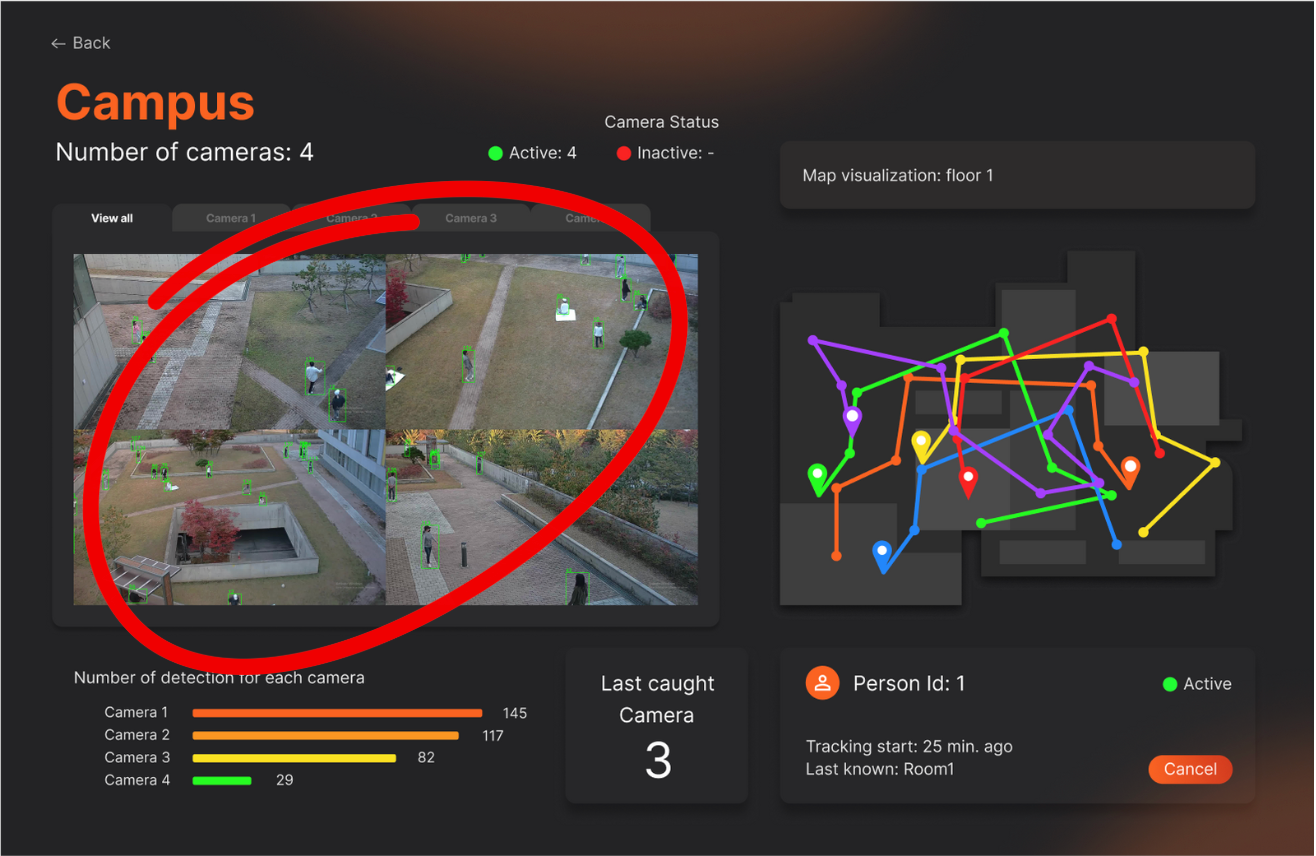
\includegraphics[width=1.0\textwidth,keepaspectratio]{JubJones-SRS/assets/jubjones/ai_mockup_bbox.png}
    \caption{AI-Annotated Multi-Camera View with Person Detection.}
    \label{fig:ai_mockup_bbox}
\end{figure}

The system leverages Artificial Intelligence primarily through an Annotate interaction style to enhance the user's ability to monitor and analyze activity across multiple camera views. In this specific mockup, the AI processes the video streams from each active camera to perform person detection.
When the AI identifies a person within a camera's field of view, it annotates the visual feed by drawing a bounding box (seen as green rectangles around individuals in the composite camera display) around that person. This direct visual annotation serves multiple purposes: it immediately draws the operator's attention to the presence and specific location of individuals, helps in quickly assessing the number of people in an area, and provides a clear visual marker for each detected person. By automatically highlighting these individuals, the AI significantly reduces the cognitive load on the human operator, who no longer needs to manually scan complex scenes. These bounding boxes are fundamental AI-generated annotations that support rapid visual assessment and are a foundational element for more complex tasks like person tracking and re-identification across different cameras, which are also hinted at by the map visualization and person ID information on the right side of the interface.

\begin{figure}[!htb]
    \centering
    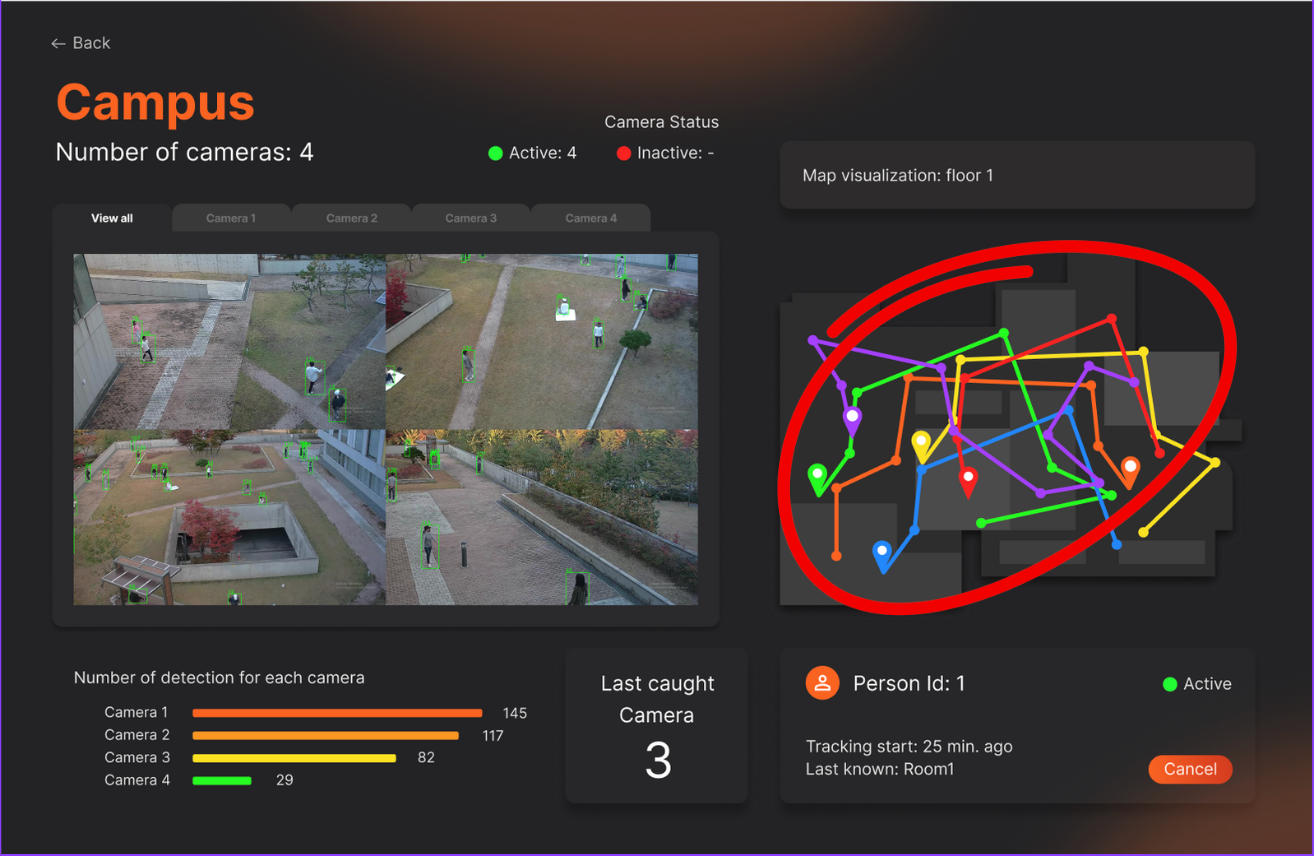
\includegraphics[width=1.0\textwidth,keepaspectratio]{JubJones-SRS/assets/jubjones/ai_mockup_map.png}
    \caption{AI-Generated Trajectory Map for Multi-Person Tracking.}
    \label{fig:ai_mockup_map}
\end{figure}

The system utilizes Artificial Intelligence in an Annotate interaction style to provide users with a comprehensive spatial understanding of movement patterns within the monitored area, as depicted in the map visualization. The AI is responsible for several complex tasks that culminate in this annotated map display.
Firstly, AI models detect individuals in various camera feeds (as seen on the left). Crucially, the AI then performs cross-camera re-identification, assigning a persistent global ID to each individual and tracking them as they move between different camera views, even if those views don't overlap or if there are temporal gaps. Simultaneously, the AI uses homography or other spatial mapping techniques to transform the 2D pixel coordinates of a detected person in a camera image into corresponding coordinates on a unified 2D floor plan or map of the environment.
The map display itself is an AI-driven annotation. The lines and markers on the map are not manually drawn but are generated by the AI, representing the historical and current paths of tracked individuals. Each distinct color typically corresponds to a unique global person ID, allowing operators to visually differentiate and follow the movements of multiple people simultaneously. The location markers (pins) indicate the last known positions or significant points along these paths. This annotated map provides powerful insights into pedestrian flow, area usage, and individual trajectories, all derived from the AI's continuous processing and interpretation of multi-camera surveillance data. It transforms raw video into a spatially coherent and easily digestible overview of activity.

\begin{figure}[H]
    \centering
    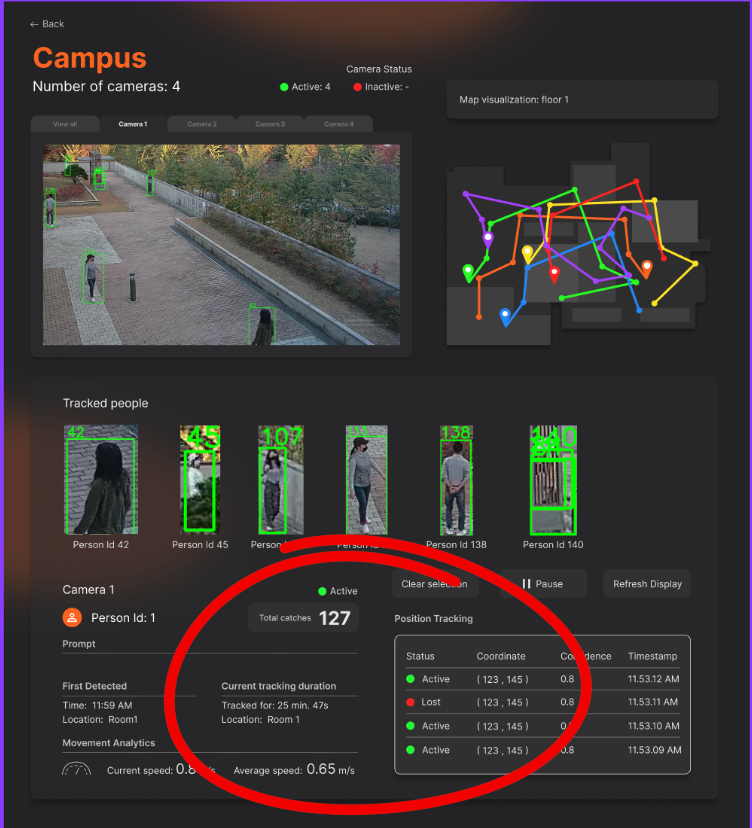
\includegraphics[width=1.0\textwidth,keepaspectratio]{JubJones-SRS/assets/jubjones/ai_mockup_data.png}
    \caption{Detailed AI-Annotated Tracking Information and Movement Analytics.}
    \label{fig:ai_mockup_data}
\end{figure}

The system employs Artificial Intelligence in an Annotate interaction style to provide users with detailed, actionable insights into the behavior and history of tracked individuals, as shown in the focused panel for "Person Id: 1". This detailed view is a direct result of the AI's continuous processing and analysis of surveillance data.
The AI is responsible for initially detecting the person in a camera feed, assigning them a unique ID (Person Id: 1), and then persistently tracking their movements across time and potentially across different cameras. The "Position Tracking" table is populated by AI-derived annotations:
\begin{itemize}
    \item   \textbf{Status (Active/Lost):} The AI determines if the person is currently visible or if their track has been temporarily lost.
    \item   \textbf{Coordinate:} The AI calculates the person's location (likely map coordinates derived via homography from camera views).
    \item   \textbf{Confidence:} The AI provides a confidence score for its detection and tracking at each point in time.
    \item   \textbf{Timestamp:} Each recorded state is timestamped, allowing for a chronological review of the person's movements. 
\end{itemize}
Furthermore, the "Movement Analytics" section, displaying "Current speed" and "Average speed," is also an AI-driven annotation. The AI calculates these metrics based on the changes in the person's position over time. Information like "First Detected," "Current tracking duration," and "Location" are all data points collated and maintained by the AI's tracking algorithms.
In essence, the AI transforms raw video data into a structured, quantitative, and qualitative summary for each tracked person. This annotated information allows operators to quickly understand a person's history, assess their current state, and gain insights into their movement patterns without needing to manually review hours of footage or perform complex calculations. The AI annotates the interface with this rich data, empowering the user with a deeper understanding of the events unfolding in the monitored environment.

\section{(Optional) Deployment Strategy}
\label{section:deployment} % Kept original unique label
This section outlines the strategy for deploying the AI components of the \usevar{\srsTitle} system and integrating them within the overall software architecture to ensure a robust and scalable solution.

\subsection{Deployment Plan}
\label{subsection:deployment_plan} % Kept original unique label
\begin{itemize}
    \item \textbf{Deployment Location:}
        The AI components, specifically the object detection (Faster R-CNN) and re-identification (OSNet) models, are integrated directly within the system's core \textbf{Backend} service. This Backend service, along with the entire system infrastructure (Frontend server, databases, caching, reverse proxy), is designed to be deployed in a \textbf{Cloud} environment. This approach leverages cloud scalability and managed services, facilitating access to necessary computational resources (including potential GPU instances for the Backend) and centralized data storage (AWS S3 for image data).

    \item \textbf{AI Communication with System Components:}
        The AI models (Faster R-CNN, OSNet) run embedded within the Python-based FastAPI Backend process. Communication between the AI logic and other system parts occurs as follows:
        \begin{itemize}
            \item \textbf{Internal Calls:} The main FastAPI application logic directly invokes the PyTorch models (loaded in memory) for detection, tracking, and feature extraction using standard Python function calls. Image preprocessing is handled internally using OpenCV.
            \item \textbf{Backend to Data Storage/Cache:} The Backend interacts with Redis (for real-time state caching and Re-ID gallery lookups) and TimescaleDB/PostgreSQL (for storing historical tracking events and embeddings) through standard database client libraries within the Python environment.
            \item \textbf{Backend to Frontend (Real-time):} Processed tracking results, including AI-generated bounding boxes, global IDs, and map coordinates, are pushed from the FastAPI Backend to the React Frontend using \textbf{WebSocket} connections. This allows for real-time visualization updates on the user interface. The WebSocket connection is managed by FastAPI and proxied through Nginx.
            \item \textbf{Frontend to Backend (Control/Queries):} User interactions triggering playback control (start, stop, seek) or requests for historical/analytical data are sent from the React Frontend to the FastAPI Backend primarily via \textbf{RESTful APIs} (implicitly provided by FastAPI for specific endpoints) or potentially dedicated messages over the established WebSocket connection. All external communication first passes through the Nginx reverse proxy.
        \end{itemize}

    \item \textbf{Tools and Frameworks Used:}
        The deployment relies on the following key technologies as described in the system architecture:
        \begin{itemize}
            \item \textit{Containerization \& Orchestration:} \textbf{Docker} for containerizing all services (Backend, Frontend server, Databases, etc.), and \textbf{Kubernetes} or \textbf{Docker Compose} for orchestrating the deployment and management of these containers.
            \item \textit{Backend Framework:} \textbf{FastAPI} (Python) serves as the core backend framework, hosting the API endpoints, WebSocket logic, and orchestrating the AI processing pipeline.
            \item \textit{AI Models \& Libraries:} \textbf{PyTorch} as the deep learning framework, with specific models like \textbf{Faster R-CNN} (for detection/tracking) and \textbf{OSNet} (for Re-ID). \textbf{OpenCV} is used for image manipulation.
            \item \textit{Frontend Framework \& State Management:} \textbf{React} for building the user interface and \textbf{Zustand} for managing frontend state.
            \item \textit{Data Storage \& Caching:} \textbf{AWS S3} for raw image data storage, \textbf{Redis} for caching, and \textbf{TimescaleDB} (built on \textbf{PostgreSQL}) for historical time-series tracking data.
            \item \textit{Reverse Proxy:} \textbf{Nginx} acts as the entry point, handling request routing, load balancing (if scaled), serving static frontend files, and proxying WebSocket connections.
            \item \textit{Monitoring \& Logging:} \textbf{Prometheus} for metrics collection, \textbf{Loki} for log aggregation (with agents like \textbf{Promtail}), and \textbf{Grafana} for visualization dashboards.
        \end{itemize}

    \item \textbf{System Qualities (Reliability, Security, Maintainability, Scalability):}
        The deployment strategy incorporates several elements to ensure key system qualities:
        \begin{itemize}
            \item \textit{Reliability:} Container orchestration (Kubernetes/Compose) enables automatic restarts of failed containers. The monitoring stack (Prometheus, Grafana, Loki) provides visibility into system health, allowing for proactive issue detection and resolution. Redundancy can be built into the database and caching layers depending on cloud provider options and configuration.
            \item \textit{Security:} The \textbf{Nginx} reverse proxy acts as a single entry point, allowing for centralized implementation of security measures like HTTPS termination, rate limiting, and access controls. Containerization isolates services, reducing the attack surface. Network policies within the orchestrator (Kubernetes) can further restrict communication between services. Secure access to AWS S3 and databases relies on proper IAM roles and credentials management.
            \item \textit{Maintainability:} Containerization with \textbf{Docker} ensures consistent environments across development, testing, and production, simplifying updates and dependency management. Defining infrastructure as code (e.g., Docker Compose files, Kubernetes manifests) makes the deployment reproducible and easier to modify. The modular architecture with clear service boundaries (Frontend, Backend, Database, Cache) aids in isolating and managing components. Centralized logging (Loki) and metrics (Prometheus) simplify troubleshooting.
            \item \textit{Scalability:} Deploying in the \textbf{Cloud} provides access to scalable resources. \textbf{Kubernetes} (or potentially Docker Swarm with Compose) allows for horizontal scaling of stateless services like the FastAPI Backend and the Nginx proxy by running multiple container instances behind a load balancer (handled by Nginx or the orchestrator's ingress controller). The database (TimescaleDB) and cache (Redis) can often be scaled independently using cloud provider services or specific clustering features. The processing pipeline itself, handling data sequentially, can be parallelized across multiple cameras if backend resources allow or scaled horizontally if processing independent time chunks is feasible.
        \end{itemize}
\end{itemize}

\subsection{Proof of Concept}
\label{subsection:poc}
The Proof of Concept (PoC) for the AI component focused on validating the feasibility, performance, and integration of the selected person detection model, which forms a critical foundation for the \usevar{\srsTitle}'s multi-camera tracking capabilities.

\textbf{Model Development and Training Strategy:}
The Faster R-CNN model, featuring a ResNet-50 backbone and Feature Pyramid Network (FPN), was selected as the baseline person detection model for the system. This decision was based on a comparative analysis of performance metrics, particularly its strong performance on medium-sized objects and high recall, as detailed in Section \ref{subsection:model_selection_experimentation}.
The model was developed using the PyTorch deep learning framework and TorchVision library. It was fine-tuned on the MTMMC dataset (further described in Section \ref{subsection:dataset-information}), which provides diverse and challenging scenarios representative of the target campus and factory environments. The training pipeline, as outlined in Section \ref{subsection:model_training_impl}, incorporated several key stages:
\begin{itemize}
    \item Standardized data preprocessing, including image resizing, color conversion, tensor transformation, and normalization using ImageNet statistics.
    \item Initialization with pre-trained weights from the ImageNet dataset to leverage learned features and expedite convergence.
    \item Modification of the model's classification head (box predictor) to specifically cater to the 'person' class (and background), aligning with the system's objective.
    \item Utilization of MLflow for systematic tracking of experiments, parameters, and results during the model development lifecycle.
\end{itemize}

\textbf{Testing and Validation Approach:}
The performance of the person detection model was rigorously evaluated through:
\begin{itemize}
    \item \textbf{Quantitative Evaluation:} The model was tested against a dedicated validation split of the MTMMC dataset. Performance was measured using standard COCO-style mAP metrics, as detailed in Section \ref{subsection:model_training_impl} and summarized in Table \ref{tab:model_performance_comparison}.
    \item \textbf{Unit Testing:} Key software components integral to the training and evaluation pipeline, such as dataset loading mechanisms, metric calculation functions, model instantiation logic, and utility functions, were subjected to unit tests using pytest. This ensured the reliability and correctness of the underlying codebase, as described in the "Unit Testing" part of Section \ref{subsection:model_training_impl}.
\end{itemize}

\textbf{Performance Results and Metrics:}
The comparative performance of the selected Faster R-CNN model against other candidate architectures is presented in Table \ref{tab:model_performance_comparison}. For the 'person' class, the Faster R-CNN model achieved:
\begin{itemize}
    \item An `eval_ap_person` (Mean Average Precision for the 'person' class) of 0.320.
    \item An overall `eval_map` of 0.320.
    \item A notable `eval_map_medium` score of 0.255, indicating strong performance on medium-sized objects, which are critical in many surveillance scenarios.
    \item The highest `total_person_detections` count of 190,884 among the compared models, suggesting superior recall capabilities crucial for minimizing missed detections in a tracking pipeline.
    \item An acceptable processing speed of 10.42 FPS for the backend batch processing context.
\end{itemize}
Initial sample runs, detailed in Section \ref{subsection:model_training_impl} (see Table \ref{tab:fasterrcnn_sample_results}), demonstrated the model's learning capability even on a subset of data (e.g., `eval_map` of 0.6522), providing early validation and direction for subsequent, more extensive fine-tuning and experimentation.

\textbf{Demonstration on Representative Data and Scenarios:}
The practical applicability and interpretability of the chosen Faster R-CNN model were demonstrated through:
\begin{itemize}
    \item \textbf{Qualitative Visualizations:} Grad-CAM heatmaps, presented in Section \ref{subsection:model_explainability} (Figures \ref{fig:gradcam_example1}, \ref{fig:gradcam_example2}, and \ref{fig:gradcam_example3}), illustrate the model's ability to focus on relevant image regions (e.g., torso, head) when detecting persons in varied scenes (factory and campus environments) from the MTMMC dataset. This confirmed that the model learns meaningful features for person identification.
    \item \textbf{Comparative Performance Justification:} As discussed in Section \ref{subsection:model_selection_experimentation}, while Faster R-CNN was not universally superior across all metrics (e.g., RTDETR-X had slightly higher overall mAP and speed), its robust performance on medium-sized objects, higher detection count (recall), and observed qualitative stability (less prone to NMS issues compared to some alternatives during initial tests) made it the preferred baseline model for this system.
\end{itemize}
This PoC effectively demonstrates that the chosen AI model, training methodology, and testing procedures yield a person detection component capable of meeting the foundational requirements of the \usevar{\srsTitle}. The achieved performance, validated through both quantitative metrics on representative datasets and qualitative analysis of its behavior on real-world like images, confirms the viability of the AI design for subsequent integration into the broader tracking and re-identification pipeline.


\subsection{(Optional) Reflection and Future Development}
\label{section:reflection} % Kept original unique label
This section is designated for a comprehensive reflection on the project's development process, outcomes, and lessons learned, alongside an outline of potential avenues for future development and enhancements. The content for this section will be thoughtfully prepared and included upon the final completion of the project.